%%%%%%%%%%%%%%%%%%%%%%%%%%%%%%%%%%%%%%%%%%%%%%%%%%%%%%%%%%%%%%%%%%%%%%
% How to use writeLaTeX:
%
% You edit the source code here on the left, and the preview on the
% right shows you the result within a few seconds.
%
% Bookmark this page and share the URL with your co-authors. They can
% edit at the same time!
%
% You can upload figures, bibliographies, custom classes and
% styles using the files menu.
%
% If you're new to LaTeX, the wikibook is a great place to start:
% http://en.wikibooks.org/wiki/LaTeX
%
%%%%%%%%%%%%%%%%%%%%%%%%%%%%%%%%%%%%%%%%%%%%%%%%%%%%%%%%%%%%%%%%%%%%%%
\documentclass{tufte-handout}

%\geometry{showframe}% for debugging purposes -- displays the margins

\usepackage{amsmath}

% Set up the images/graphics package
\usepackage{graphicx}
\setkeys{Gin}{width=\linewidth,totalheight=\textheight,keepaspectratio}
\graphicspath{{graphics/}}

\title{Stata Lab 3: High Frequency Checks}
\author{Benjamin Daniels \\ bdaniels@worldbank.org}
% \date{24 January 2009}  % if the \date{} command is left out, the current date will be used

% The following package makes prettier tables.  We're all about the bling!
\usepackage{booktabs}

% The units package provides nice, non-stacked fractions and better spacing
% for units.
\usepackage{units}

% The fancyvrb package lets us customize the formatting of verbatim
% environments.  We use a slightly smaller font.
\usepackage{upquote}
\usepackage{fancyvrb}
\fvset{fontsize=\normalsize}
\renewcommand{\FancyVerbFormatLine}{\color{violet}}
\DefineShortVerb{\|}

% Small sections of multiple columns
\usepackage{multicol}

% Provides paragraphs of dummy text
\usepackage{lipsum}

% These commands are used to pretty-print LaTeX commands
\newcommand{\doccmd}[1]{\texttt{\textbackslash#1}}% command name -- adds backslash automatically
\newcommand{\docopt}[1]{\ensuremath{\langle}\textrm{\textit{#1}}\ensuremath{\rangle}}% optional command argument
\newcommand{\docarg}[1]{\textrm{\textit{#1}}}% (required) command argument
\newenvironment{docspec}{\begin{quote}\noindent}{\end{quote}}% command specification environment
\newcommand{\docenv}[1]{\textsf{#1}}% environment name
\newcommand{\docpkg}[1]{\texttt{#1}}% package name
\newcommand{\doccls}[1]{\texttt{#1}}% document class name
\newcommand{\docclsopt}[1]{\texttt{#1}}% document class option name

\begin{document}

\maketitle% this prints the handout title, author, and date

\begin{marginfigure}%
  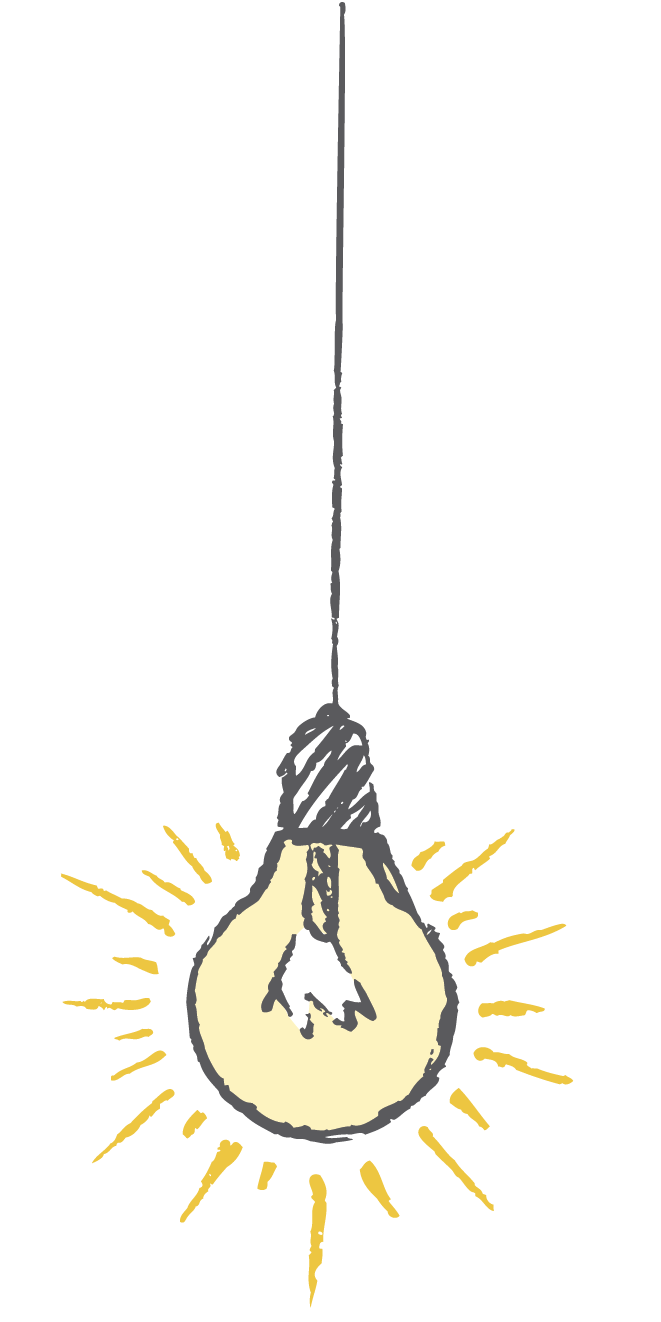
\includegraphics[width=\linewidth]{light.png}
\end{marginfigure}

\begin{abstract}
High Frequency Checks (HFC) can support the data collection process
through the timely verification of incoming raw data.
This can allow for the correction of survey programming,
discussion with enumerators, and the rapid cleaning of data.
In this lab, we will practice setting up and running HFCs.

\bigskip\noindent \textbf{Exercise Objectives}:
\begin{enumerate}
  \item Set up and run high frequency checks
\end{enumerate}
\end{abstract}

%\printclassoptions
\section{What are high frequency checks?}

High-frequency checks takes in the raw data on a daily basis,
assesses its quality using Stata dofiles
and produces output excel spreadsheets.
Some key categories for verification are:

\begin{itemize}
  \item Check that there are no duplicates.
  \item Check that all surveys have consent.
  \item Check that certain variables have no missing values.
  \item Check that follow up records match master
  \item Check skip patterns and survey logic.
  \item Check for variables that contain only missing values.
  \item Check hard/soft constraints for continuous variables.
  \item Check specify other variables for recodes or recategorizations.
  \item Check that continuous variables have no outliers.
\end{itemize}

Furthermore, data quality checks often include the following enumerator and research checks:

\begin{itemize}
  \item Check the percentage of “don’t know” and “refusal” values for each variable by
enumerator
  \item Check the percentage giving each answer for key filter questions by enumerator
  \item Check the percentage of survey refusals by enumerator
  \item Check the number of surveys per day by enumerator
  \item Check average interview duration by enumerator
  \item Check the duration of consent by enumerator
  \item Check the duration of other (anthropometrics, games, etc.)
\end{itemize}

\section{Running custom high-frequency checks}

Open your |/DataWork/| folder for the full training.
It should have subfolders for each of the Labs;
if it does not, use |iefolder| to create the subfolder for |Lab3| now.
You will find a raw data file, |endline_data_raw_nodup.dta|
in the public Field Coordinator Training folder.
Save this dataset to |/Lab3/|.
Get the template |lab4-HFC-template.do| from the public folder.
This provides some basic setup for the command |putexcel| that can be very useful. Note: |putexcel| syntax is relatively new and will not work like this on Stata versions before 14.0.

First, adapt the template to load the correct data,
and point the |set putexcel| command at your outputs folder.
The next part of the template will clean up the timing variables in this survey.
Take a minute to figure out how these work if you like,
and feel free to adapt for future use.
Then, we’ll get started with the checking.

\subsection{Checking survey durations}
Calculate the duration of each survey in minutes
using the |start_clock| and |end_clock| variables.
Do |help datefime| if you need to figure out how to handle
the units on these (they are typically in milliseconds).
Figure out which surveys are very short:
take the bottom fifth percentile of surveys using |sum , d| and |return list|.
Generate a variable called |issue| which notes the problem with these,
and a variable called |variable| which flags the variable
on which the issue was noted.

Export the |enumerator| variables, the variable name, and the issue
to the sheet that is initiated at the beginning of the template
using |putexcel| or |export excel|.

\subsection{Identify households with no plots}
This is an agriculture survey, so finding households with missing data
is key to double check.
Mark out observations for which |numplots| is equal to zero.
If there are, create the |variable| and |issue| labels as below
and export these to the same sheet, so the total number of issues increases.
If you are running into conflicts,
think about using |preserve| and |restore|
or reloading your data strategically for each check.)

\subsection{Identify farmers with no crops}
In this survey, crops are identified in the variables with names
of the form |ag9n_16*|. Examine those variables as you like
with commands like |sum| and |tab|.
Keep the observations for which the total number of crops is zero,
and flag and export those as in the previous two parts.
Note: since some will have missing data, you will need to use |egen| here,
probably with the |rowtotal()| function.
How is this different from the “+” operator?

\subsection{Identify outliers in equipment rent}
Identify the households that rent equipment |exp_18|.
Find those that have total expenditures above 100,000 francs, flag them,
and export them to the same sheet.
When you are done you should have a sheet of data issues.
your dofile might look like the one below.

\section{The \texttt{ieduplicates} and \texttt{iecompdup} commands}

The \texttt{ieduplicates} and \texttt{iecompdup} commands
are used to identify and resolve duplicates in raw survey data while data collection is ongoing.
\texttt{ieduplicates} is meant to be used directly after importing raw data from,
for example, a server used in survey data collection. The command does two high-level tasks.
It outputs a report of all the duplicates (the report can be used for correcting the duplicates)
and it removes the duplicates from the data set until they are resolved.

Duplicates are removed because many other quality checks require unique IDs
in the dataset and cannot be completed with the data in that state;
yet resolving duplicates is often among the slowest correction processes.
For example, if a household with ID \texttt{A123456} was selected for back checks,
but you incorrectly have two observations that were given the ID \texttt{A123456},
then it is better to resolve that duplicate first (you can use the report for this)
before trying to run the back check test on either of the observations the ID potentially represents.
It is important that you make sure to not overwrite the original raw data
with the data set where \texttt{ieduplicates} has removed the duplicates
as you would lose that data. To avoid this,
save the dataset with removed duplicates with a different name.

Meanwhile, \texttt{iecompdup} helps identify the reason for the duplicates so they can be resolved.
The decision on how to correct a duplicate is always a qualitative decision.
\texttt{iecompdup} compares the duplicated entries variables by variables. 
The output format can be selected by the user, depending on their decision process.
See below for instructions on how to interpret the output of \texttt{iecompdup}.
The intended work flow is as follows:

\begin{enumerate}
    \item Run \texttt{ieduplicates} on the raw data. If there are no duplicates, you are done.
    \item If there are duplicates, use \texttt{iecompdup} on any duplicates identified.
    \item Enter the corrections identified with \texttt{iecompdup} to the duplicates in the report outputted by \texttt{ieduplicates}.
    \item After entering the corrections, save the report in the same location with the same name.
    \item Run \texttt{ieduplicates} on the raw data again. The corrections you have entered will be applied, and only duplicates that are still not resolved are removed this time. Note that the raw data is unchanged, and therefore the report leaves a record of how all duplicates were resolved in the creation of the final dataset.
    \item Repeat these steps every time you get new data. Our recommendation is that this is done every day that you have new data.
\end{enumerate}

\subsection{Listing and resolving duplicate observations with \texttt{ieduplicates}}

These instructions are meant to help you understand how to use \texttt{ieduplicates} in Stata.
As inputs, \texttt{ieduplicates} requires, first, a singular unique ID variable,
which, if repeated, would be an unacceptable duplicate in the dataset.
This variable can be string or numeric.
It then requires a folder in which to export the duplicates report in Excel format.
Finally, it requires a unique observation variable by which to identify actual observations in the dataset --
software like SurveyCTO create these automatically, and they are commonly called \texttt{KEY};
other data collection methods should have such an identifier built into their data collection process,
as solutions such as using \texttt{\_n} will usually not be sufficient.

The reason a folder is accepted as the input rather than a target filepath is twofold.
First, the filename itself is standardized.
Second, since the expectation is that the command will be used frequently,
it also manages a subfolder called \texttt{/Daily/} where it saves
dated backup reports whenever it is re-run, in case the main report or any contents are deleted.
(If two different reports are generated the same day,
then the first one will be overwritten by the second.)
To restore a backup version, simply copy it out of the Daily folder
and remove the date from the name.

Inside the report, you can indicate corrections which resolve the duplicated observations.
By this method, the report becomes a permanent documentation on how
duplicated IDs were resolved from the raw data.
There are three options for resolution offered as columns in the report:
\textit{correct}, \textit{drop}, and \textit{newID}.
If you want to keep one duplicate and drop another one as they are double recordings
of the same observation, then write ``yes'' in the \textit{correct} column
for the observation with the {\it key\_variable} you want to keep,
and ``yes'' in the \textit{drop} column for the one you want to drop.
If you want to keep one duplicate and assign a new ID to another duplicate,
then you write ``yes'' in the \textit{correct} column for the observation you want to keep,
and the correct new ID value in the \textit{newID} column for the observation
that you want to assign a new ID to. You can combine these two methods
if you have many duplicates with the same ID. Note that you must
always indicate which observation to keep for each duplicate set.
After you have entered your corrections, save the file and run
\texttt{ieduplicates} again to apply the corrections --
\texttt{ieduplicates} will automatically recognize that a completed report is already there.

\subsection{Analyzing duplicate observations with \texttt{iecompdup}}

\texttt{ieduplicates} only identifies duplicates but gives you no help in how to resolve them.
That is what \texttt{iecompdup} does. \texttt{iecompdup} requires as inputs the intended unique ID variable
(the same one as in \texttt{ieduplicates}) and the ID value you wish to examine.

If you have several pairs or groups of duplicates you will have to run this command multiple times.
This is because \texttt{iecompdup} can only be run on two duplicates at a time:
the multi-way relationships among duplicate groups larger than two may be too complex to be informative.
Therefore it picks the two first observations in the sort order each time by default,
and you need to change the sort order if you want to change which two duplicates are compared.
\texttt{iecompdup} gives you a warning if this is the case,
and you may suppress this warning by using the option \texttt{more2ok}.

The output for \texttt{iecompdup} is information on the variables where the duplicate pair
has identical values and where the duplicate pair has different values.
The section below outlines three types of duplicates that we have identified
as reasons for duplicates when working with SurveyCTO, and how \texttt{iecompdup}
can be used to identify which of these cases applies to the duplicate pair.
The general picture should be the same even if you are using a different software,
but some details might be different. No output from \texttt{iecompdup}
can guarantee any of the cases below, but most of the times the output
will still be conclusive for one of the three cases.

\begin{itemize}
    \item Type 1: Double submission of the same observation, with the same data.
    \item Type 2: Double submission of the same observation, but with modified data.
    \item Type 3: Incorrectly assigned ID.
\end{itemize}


Type 1 error is often a consequence of a circumstance like poor internet connection during data collection.
If a submission of data is interrupted before it is completed in some softwares,
then the server may still save that incomplete data.
When the server receives a second submission, it saves both submissions,
as it impossible for the server to know if two submissions
or changes made between them were intentional.
In \texttt{iecompdup} this case would result in very few variables being different
and the variables that differ are mostly submission metadata such as submission time
or submission ID (the \texttt{KEY} variable in SurveyCTO).
If no media files (audio, images, monitoring) were used and only metadata that differs,
it does not matter which observation that is kept,
but it is good practice to keep the one submitted most recently.
However, when a submission is interrupted it is usually media files such as audio or video
that were not uploaded correctly. Those files do not come up as variables in Stata,
only the name of the file, so only submission metadata variables will differ.
The filename variable will differ, and sometimes that name value is submitted
even when the file is not. When both duplicates have filenames it
does not matter which duplicate you keep, but if only one has the filename
you should keep that observation.

Case 2 errors are possible but rare in most data collection software,
as it is bad practice to allow multiple complete observations with the same ID
to be validly submitted. Recent advancements in ``case management'' workflows are available
on most survey software to control this process.
However, Case 2 errors may still occur if an observation if modified after the first submission and then resubmitted.
Sometimes there is a need for modifying data already submitted;
but then it is much better practice to do so in a do-file when the data set is cleaned
(such as through ``revisions'' workflows in the survey software).
This way, the manual modifications are properly documented.
In \texttt{iecompdup} this would show up as the submission metadata differs,
and some observation data also differs.
These cases have to be manually examined and followed up
with the field team responsible for the submission to confirm which entry should be kept.

Case 3 errors can occur by mistake any time.
This can be due to typos or to protocols not being followed correctly in the field.
In \texttt{iecompdup}  this would show up as submission data differing,
as well as a many differences in survey responses.
You will need to follow up with enumerators and supervisors responsible
for this submission and assign a new ID to one of the observations
based on what you learn when investigating this case.


\begin{figure*}[h]
{\setstretch{0.7}
\VerbatimInput[frame=lines,numbers=left,label=hfc-1.do]
{../DataWork/Lab3/hfc-1.do}}
\end{figure*}

\begin{figure*}[h]
{\setstretch{0.7}
\VerbatimInput[frame=lines,numbers=left,label=hfc-2.do]
{../DataWork/Lab3/hfc-2.do}}
\end{figure*}

\begin{figure*}[h]
{\setstretch{0.7}
\VerbatimInput[frame=lines,numbers=left,label=hfc-3.do]
{../DataWork/Lab3/hfc-3.do}}
\end{figure*}

\begin{figure*}[h]
{\setstretch{0.7}
\VerbatimInput[frame=lines,numbers=left,label=hfc-4.do]
{../DataWork/Lab3/hfc-4.do}}
\end{figure*}

Thanks to the template creators.\cite{tuftelatex}

\bibliography{sample-handout}
\bibliographystyle{plainnat}

\end{document}
